\chapter{Lec 04-05 - Learning With Gradient Descent}

\section{Gradient-based optimization}
In machine learning we want to maximize/minimize an \textbf{objective function}. This is done by minimizing an \textbf{error function}, which is a measure of the committed error. This optimization problem can be solved exploiting the concepts of derivative and \textbf{gradient}.\newline\newline 
\textbf{Derivative:}\newline
The derivative $f'$ tells us the slope of a function $f$ at any point $x$.
\[f'(x) = lim_{\epsilon \rightarrow 0}\frac{f(x + \epsilon) - f(x)}{\epsilon} \quad \epsilon > 0\]
Given a point:
\begin{itemize}
    \item Positive derivative means that the function increases at that point
    \item Negative derivative means that the function decreases at that point.
    \item Null derivative means that there is a stationary point (minimum, maximum or saddle point).
\end{itemize}
In order to minimize a function in 1 variable, we have to move in the direction \textbf{opposite} to the function derivative.\newline\newline
\textbf{Gradient} is the generalization of derivative with respect to a vector of input variables. In vector calculus, the gradient of a scalar-valued differentiable function $f: \mathbb{R}^{n} \rightarrow \mathbb{R}$ is a vector-valued function $\nabla f: \mathbb{R}^{n} \rightarrow \mathbb{R}^{n}$ whose value at point $p$ is the vector whose components are the partial derivatives of $f$ at $p$.\newline\newline
The gradient vector can be interpreted as the direction and rate of fastest increase of the function. The gradient is the zero vector at a point if and only if the point is a stationary point.
\subsection{Multivariate calculus}
Let's consider a function $f: \mathbb{R}^{2} \rightarrow \mathbb{R}$. It is a function of 2 variables $x_{1}, \,\, x_{2}$ where $x_{1}(t),\,\, x_{2}(t)$ are 2 functions themselves. The derivative of $f$ with respect to $t$ is defined as follows:
\[\frac{d\,f}{d\,t} = \frac{\partial f}{\partial x_{1}}\frac{\partial x_{1}}{\partial t} + \frac{\partial f}{\partial x_{2}}\frac{\partial x_{2}}{\partial t}\]
We can write the formula above in a more convenient way using vectors multiplications:
\[
    \begin{bmatrix}
        \frac{\partial f}{\partial x_{1}}, & \frac{\partial f}{\partial x_{2}} 
    \end{bmatrix}
    \cdot
    \begin{bmatrix}
        \frac{\partial x_{1}(t)}{\partial t}\\
        \vspace{1pt}
        \frac{\partial x_{2}(t)}{\partial t}\\
    \end{bmatrix}
\]
Note that the first term is the gradient of $f$ $\nabla_{\Vec{x}} f$. Note also that $\frac{\partial x_{1}(t)}{\partial t}$ is $\nabla_{t}x_{1}$, and $\frac{\partial x_{2}(t)}{\partial t}$ is $\nabla_t x_2$. We can define $X: \mathbb{R} \rightarrow \mathbb{R}^{2}$ as the following vector:
\[
    \begin{bmatrix}
        x_1 \\
        x_2
    \end{bmatrix}
\]
where $x_1: \mathbb{R} \rightarrow \mathbb{R}$ and $x_2: \mathbb{R} \rightarrow \mathbb{R}$\newline\newline
\textbf{Example:}\newline
$f(x_1, x_2) = x_1^{2} + 2x_2$ where $x_1 = sin(t), \,\, x_2 = cos(t)$
\[
    X(t) = 
    \begin{bmatrix}
        sin(t) \\
        cos(t)
    \end{bmatrix}
\]
\begin{itemize}
    \item $\frac{\partial f}{\partial x_1} = 2x_1$
    \item $\frac{\partial f}{\partial x_2} = 2$
    \item $\frac{\partial x_1}{\partial t} = cos(t)$
    \item $\frac{\partial x_2}{\partial t} = - sin(t)$
\end{itemize}
\[\frac{d \,f}{d\,t} = 2x_1\,cos(t) + 2\,(-sin(t))\]
\[= 2 \, sin(t)cos(t) - 2 \, sin(t)\]
We can do the same thing in matrix notation:
\[\frac{d \, f}{d \, t} = 
    \begin{bmatrix}
        2x_1, & 2
    \end{bmatrix}
    \cdot
    \begin{bmatrix}
        cos(t) \\
        - sin(t)
    \end{bmatrix}
    = 2 \, sin(t)cos(t) - 2 \, sin(t)
\]
\textbf{Example with more than 1 variable:}\newline
Given a function $f(x_1, x_2) = x_1^{2} + 2x_2$, let $g(s, t)$ be the following function:
\[
    g(s, t) = 
    \begin{bmatrix}
        s \cdot sin(t) \\
        s \cdot cos(t)
    \end{bmatrix}
\]
where $g_1 = s \cdot sin(t), g_2 = s \cdot cos(t)$. Let $h$ be the composition between $f$ and $g$:
\[h = f \circ g\]
We want to compute $\frac{d \, h}{d\,(s,t)}$
\[
    \frac{d \, h}{d\,(s,t)} = \frac{\partial f}{\partial \Vec{y}} \cdot \frac{\partial \Vec{y}}{\partial (s, t)} = 
    \begin{bmatrix}
        2x_1, & 2
    \end{bmatrix}
    \cdot
    \begin{bmatrix}
        \frac{\partial g_1}{\partial s}, & \frac{\partial g_1}{\partial t} \\
        \vspace{2pt}\\
        \frac{\partial g_2}{\partial s}, & \frac{\partial g_2}{\partial t}
    \end{bmatrix}
\]
where $\Vec{y} = g(s,t)$
\[
    \frac{d \, h}{d\,(s,t)} =
    \begin{bmatrix}
        2x_1, & 2
    \end{bmatrix}
    \cdot
    \begin{bmatrix}
        sin(t), & s \cdot cos(t)\\
        \vspace{1pt}\\
        cos(t), & -s \cdot sin(t)
    \end{bmatrix}
\]
The collection of all first-order partial derivatives of a vector-valued function $f: \mathbb{R}^n \rightarrow \mathbb{R}^m$ (function $g$ in this case) is called the \textbf{Jacobian Matrix}.

\subsection{Second-order methods}
So far, we have discussed gradients, i.e., first-order derivatives. Sometimes, we are interested in derivatives of higher order. Consider a function $f: \mathbb{R}^2 \rightarrow \mathbb{R}$ of two variables $x, y$.We use the following notation for higher-order partial derivatives (and for gradients):
\begin{itemize}
    \item $\frac{\partial^2 f}{\partial x^2}$ is the second partial derivative of $f$ with respect to $x$.

    \item $\frac{\partial^2 f}{\partial x \partial y}$ is the partial derivative obtained by first partial differentiating with respect to $x$ and then with respect to $y$.
\end{itemize}
The \textbf{Hessian} is the collection of all second-order partial derivative. Generally, for $\textbf{x} \in \mathbb{R}^n$ and $f: \mathbb{R}^n \rightarrow \mathbb{R}$, the Hessian is an $n \times n$ matrix. The Hessian measures the curvature of the function locally around $(x, y)$. If $f: \mathbb{R}^n \rightarrow \mathbb{R}^m$ is a vector field, the Hessian is a $(m \times n \times n)$-tensor. In general, Second order derivatives measure the curvature of a function (concave, convex).
\begin{center}
    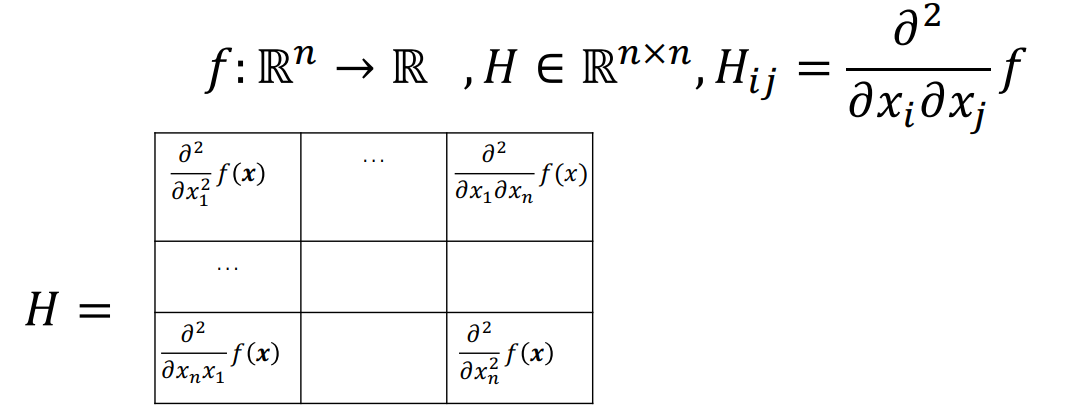
\includegraphics[scale=0.6]{images/hessian.png}
\end{center}
The \textbf{condition number} is the ratio of the maximum and minimum nonzero
eigenvalues of the Hessian matrix. It gives information about the
curvature of a function in the different dimensions. Poorly conditioned problems are long, thin valleys (very curved in one direction, very flat in the other). 
\newline\newline
Second-order optimization algorithm (like Newton’s Method) can be used to solve poorly conditioned problems exploiting the Hessian. However, these methods are slow and therefore they are not widely used for deep learning.

\section{Gradient descent}
Let $f(\textbf{x}): \mathbb{R}^{n} \rightarrow \mathbb{R}$ be a vector-valued function, find the vector $\theta \in \mathbb{R}^{n}$ that minimizes the function $f$:
\[\theta = argmin_{\textbf{x}}f(\textbf{x})\]
This minimization problem can be solved using gradient descent. Starting from a random configuration of $\theta$, each parameter is updated in the following way:
\[\theta_{k+1} = \theta_{k} - \eta \nabla f(\theta_{k})\]
where: 
\begin{itemize}
    \item $\nabla f(\theta_{k})$ is the partial derivative of the function in $\theta_{k}$.
    \item The parameter $\eta > 0$ is known as the \textit{learning rate}. 
\end{itemize}
The derivative term $\frac{\partial}{\partial \theta_{k}}f(\theta_{k})$ can be:
\begin{itemize}
    \item $\geq 0$ it means that the function is increasing, so we are decreasing $\theta_{k}$ in the \textit{right direction}.
    \item $\leq 0$ it means that the function is decreasing, so we are increasing $\theta_{k}$ in the \textit{right direction}
\end{itemize}
If $\eta$ is too small, gradient descent can be slow. Anyway, if it is too large, it can overshoot the minimum (fail to converge).

\section{Example}
Let's consider a simple example of linear regression with a function $h_{\theta}(x) = \theta_{1}x$ and a cost function $J(\theta_{1}) = \frac{1}{2m}\sum_{i = 1}^{m}(h_{\theta}(x^{(i)}) - y^{(i)})^{2}$.
\begin{center}
    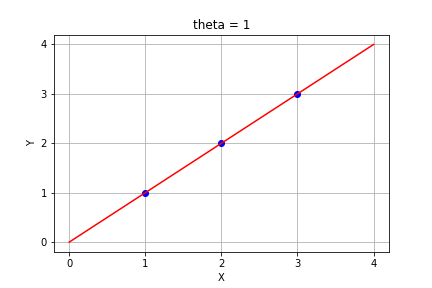
\includegraphics[scale = 0.7]{images/Simple liner reg.png}
\end{center}
As you can see from the graph above, our training set is composed by 3 points $\{(1,1), (2,2), (3,3)\}$. In this simple example the function $h_{\theta}(x)$ that perfectly fits the training set is the one with the parameter $\theta_{1} = 1$. In fact, if we compute the cost function $J(\theta_{1})$ with respect to $\theta_{1} = 1$, the result is 0 (minimized).
\[J(\theta_{1}) = \frac{1}{2m}\sum_{i = 1}^{m}(h_{\theta}(x^{(i)}) - y^{(i)})^{2}\]
\[= \frac{1}{2m}\sum_{i = 1}^{m}(\theta_{1}x^{(i)} - y^{(i)})^{2}\]
\[= \frac{1}{2m}(0+0+0)^2 = 0\]
But let's see what happens for different values of $\theta_{1}$.
\begin{itemize}
    \item $\theta_{1} = \frac{1}{2}$ $J(\theta_{1}) \approx 0.67$
    \item $\theta_{1} = 0$ $J(\theta_{1}) \approx 2.33$
    \item $\theta_{1} = -\frac{1}{2}$ $J(\theta_{1}) \approx 5.25$
\end{itemize}
\begin{center}
    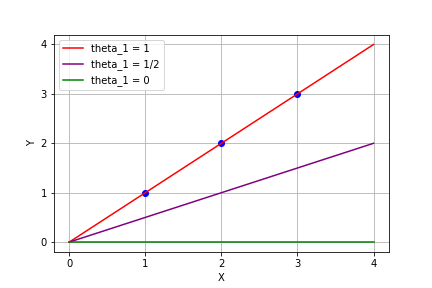
\includegraphics[scale = 0.7]{images/Simple liner reg (colors).png}
\end{center}
Now we can plot the values of $\theta_{1}$ on the \textbf{X} axis and the values of $J(\theta_{1})$ on the \textbf{Y} axis. The shape of $J(\theta_{1})$ will be the following:
\begin{figure}[h]
    \centering
    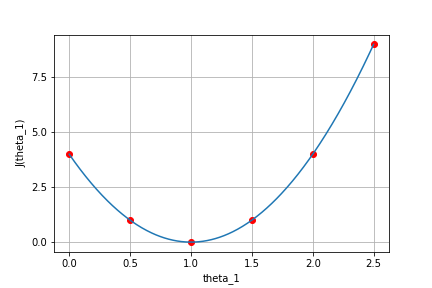
\includegraphics[scale = 0.7]{images/J.png}
    \label{Fig 1}
    \caption{Cost function J}
\end{figure}\newline
We obtain this \textbf{convex} function that has its minimum, for this specific $h_{\theta_{1}}(x^{(i)})$ and $y^{i}$, in 0. This principle is also valid for $n$-dimensional functions but the graphic representation is not that easy.\newline
We can use \textbf{gradient descent} technique in order to find $\theta_{1}$ in an automatic way.
\begin{flushleft}
    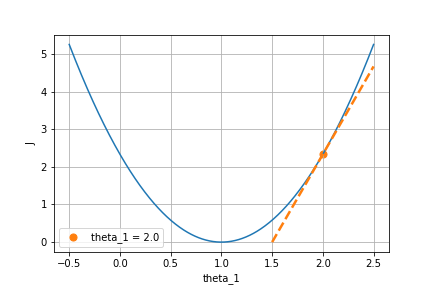
\includegraphics[scale=0.5]{images/partial derivative.png}
    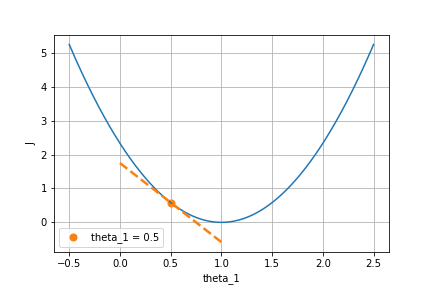
\includegraphics[scale=0.5]{images/partial derivative_1.png}
\end{flushleft}
\begin{center}
    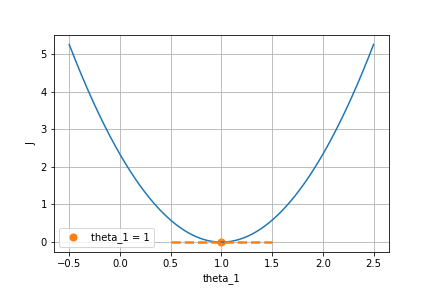
\includegraphics[scale=0.5]{images/partial derivative_2.png}
\end{center}
\textbf{Example of derivation:}\newline\newline
We want to minimize $J[\textbf{w}]$ with respect to the parameters $\textbf{w}$ using gradient descent. Let's start with the derivation of the loss function $J[\textbf{w}]$:
\[\frac{\partial J}{\partial w_{i}} = \frac{\partial}{\partial w_{i}}\left[\frac{1}{2N}\sum_{s=1}^{N}(t^{(s)} - o^{(s)})^{2} \right]\]
\[= \frac{1}{2N} \sum_{s=1}^{N}\frac{\partial}{\partial w_{i}}\left[ (t^{(s)} - o^{(s)})^{2} \right]\]
\[= \frac{1}{2N}\sum_{s=1}^{N}2(t^{(s)} - o^{(s)})\frac{\partial}{\partial w_{i}}\left[ t^{(s)} - o^{(s)}\right]\]
Note that $t^{(s)}$, which is the target value, is a constant that does not depend on $w_{i}$. So, it can be removed from the derivation.
\[= \frac{1}{N} \sum_{s=1}^{N}(t^{(s)} - o^{(s)})\left(-\frac{\partial}{\partial w_{i}}\left[\textbf{w} \cdot \textbf{x}^{(s)}\right]\right)\]
$\textbf{w} \cdot \textbf{x}^{(s)}$ = $w_{1}x_{1}^{(s)} + w_{2}x_{2}^{(s)} + ... + w_{i}x_{i}^{(s)} + ...$. The partial derivative $-\frac{\partial}{\partial w_{i}}\left[\textbf{w} \cdot \textbf{x}^{(s)}\right]$ with respect to  $w_{i}$ is equal to $x_{i}^{(s)}$ because all the other terms are constant. Therefore, the derivation becomes:
\[ = -\frac{1}{N}\sum_{s=1}^{N}(t^{(s)} - o^{(s)})x_{i}^{(s)}\]
